%%%%%%%%%%%%%%%%%%%%%%%%%%%%%%%%%%%%%%%%%%%%%%%%%%%%%%%%%%%%%%%%%%%%%%%%%%%%%%
%
% タイトル TeX用テンプレート 
% バージョン 2014-11-8 (Sat) 初版
% 作成者 Kouhei Ito
% 作成場所 野々市市中林 DeuxMKK
% 用途 2段組レポートの作成等
%
%%%%%%%%%%%%%%%%%%%%%%%%%%%%%%%%%%%%%%%%%%%%%%%%%%%%%%%%%%%%%%%%%%%%%%%%%%%%%%%%
\documentclass[a4paper]{jarticle}
\usepackage{sice-si}
\usepackage{amsmath} 
\usepackage[dvipdfmx]{graphicx}



%%%%%%%%%%%%%%%%%%%%%%%%%%%%%%%%%%%%%%%%%%%%%%%%%%%%%%%%%%%%%%%%%%%%%%%%%%%%%%%%

%%%%%%%%%%%%%%%%%%%%%%%%%%%%%%%%%%%%%%%%%%%%%%%%%%%%%%%%%%%%%%%%%%%%%%%%%%%%%%%%
\begin{document}

\title{超低重心6輪独立懸架ローバーの設計開発報告書}
\name{畠中和久(金沢工業高等専門学校)}
\etitle{hogehoge}
\ename{Kazuhisa Hatakenaka}

\abst{
自動走行するロボットには安定した走りと悪路での振動の小ささ,そしてコンパクトである事が大切になる.しかし車輪を大きくすると安定性はあるがコンパクトでない.今回参加するつくばチャレンジでは市街の走行であり,信号を渡る際のスロープや路上のコンクリート,タイルなどの凸凹道を転倒せずに安定して走行できるロボットの開発が必要である.そこで今年は重心を低くすることで走行に安定性を持たせることを目的として独立懸架の6輪のローバー型ロボットを製作する.
}

\maketitle

%%%%%%%%%%%%%%%%%%%%%%%%%%%%%%%%%%%%%%%%%%%%%%%%%%%%%%%%%%%%%%%%%%%%%%%%%%%%%%%%
\section{はじめに}
\subsection{研究背景}
茨城県南部に位置するつくば市では毎年行われる「つくばチャレンジ」というロボットの大会がある.これはつくば市内の遊歩道等の実際の環境を移動ロボットに自律走行させる大会で,地域と研究者,教育者,学生が協力して行う,人間とロボットが共存する社会のための架け橋となる大会である. 
市街走行では凸凹道やコンクリートなどでロボットに傾きが発生しそのまま転倒するケースは大いに考えられる,またその転倒によって発生する第二次災害は十分に注意しなければならない.
そこで,今回は地域住民に怪我や事故が出ないようなロボットの走行方法に注目し,”超低重心6輪独立懸架ローバー”を制作する.




\subsection{研究目的}
振動をできるだけ減らす,もしくはいなすような足回りの構造を開発する.よって全体のズレを少なくするために6輪にそれぞれサスペンションの設置をし,それが大きくかさ張らないようにする必要がある.また今回のロボットの超低重心を実現するための数値を表\ref{tab:joken} に示す


\section{目的達成の手順}
\subsection{研究の概要}
製作するロボットのはある程度の段差を超えるための上下できる機構が必要である.よって近年最も身近な上下機構を持つ機械として,車に利用されるサスペンションを参考にした.図\ref{fig:doublewish}に示すダブルウィッシュボーン式サスペンションは上下のアームとショックアブソーバ,ばねからなるもので,レーシングカーに多く使用されている.図\ref{fig:strat}に示すストラット式サスペンションと呼ばれるものはショックアブソーバとサスペンションを一体化したものをアッパーアームにしたもので,近年の車やミニ四駆などに使用されている.両方とも独立懸架で安定性や利便性に置いてはストラット式が大きく優るが,今回はコンパクトに構成することも必要なため,もともと上下アームで囲われているスペースを活かせることができそうなダブルウィッシュボーン式サスペンションを基礎として開発する.

\begin{figure}[htbt]
 \begin{center}
  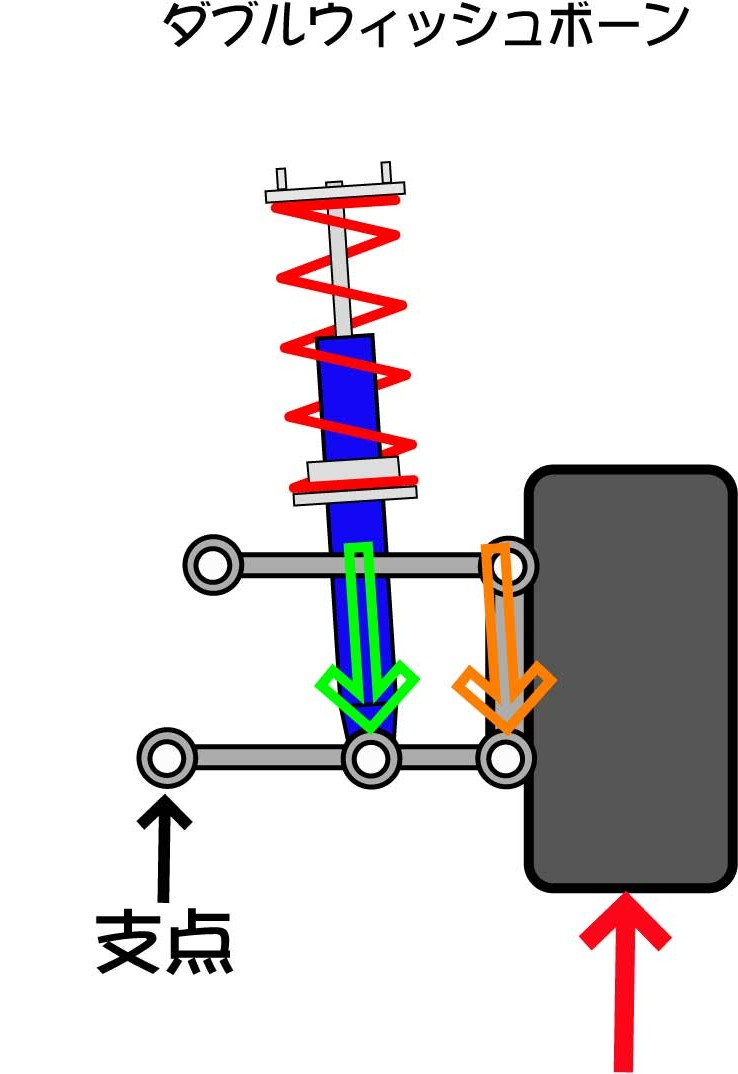
\includegraphics[width=40mm]{img/doublewish.jpg}
  \caption{ダブルウィッシュボーン式サスペンション}
  \label{fig:doublewish}%ここに文章中で使用する名前を指定する
 \end{center}
\end{figure}
\subsection{ロボットの概要図}

製作する”超低重心6輪独立懸架ローバー”(以下6輪ローバ)は図\ref{fig:rokurin}に示すとおり低重心であるがゆえにロボットそのものが平たく大きい物になる.そのままではメンテナンス性にかける他,運搬時に非常に不便なため,モータを持つドライブモジュール(以下Dモジュール)と指示塔であるコントロールモジュール(以下Cモジュール)に分解できるように設計し,分解から組み立てを容易とするようにした.つまり2つのDモジュールと1つのCモジュールからなる1つのロボットである.

\section{設計}
本項目ではサスペンションについて詳しく記す.


\subsection{サスペンションの配置}
ダブルウィッシュボーン式サスペンションは便利ではあるが問題点も目立つ.例えばばねのストロークが少ない,ストロークを大きくしようとすれば車体との接続が困難になる,決められた場所にしか設置できない等,どれもスペースが大きく関係してくる.そこで図\ref{fig:box}のように軸棒,ユニバーサルジョイント,車輪を上下のリンクと板を用いて1つの平行リンクをつくり,その平行リンクの両斜辺に2つ直接斜めに振動吸収となるばねを設置すれば車輪の径に左右されるものの従来のものよりスペースが少なく上下機構が得られるのではないかと考えた.



\subsection{ばねのストロークの算出}
図\ref{fig:bix}に平行リンクの簡易図を示す.また平行リンクが移動した際の図を図\ref{fig:rink}示す.これらの数値よりサスペンションのストロークの長さを求める.サスペンションの全体長さは斜辺に設置するため余弦定理より
\begin{eqnarray}
   AC = b^2 & = & a_1^2+c^2-2a_1c\cdot cos∠B \\
  AC = b & = & \sqrt{38^2+60^2-2\times 38\times 60\times cos90} = 71.022 ≒ 71.0 [mm]
\end{eqnarray}
となる.また今回は30[mm]程度の障害物を乗り越える想定しているため,この平行リンクが点A,Bを回転軸として点C,Dが30[mm]上昇した際の平行四辺形の斜辺AC'を求める必要がある.平行リンクが移動してできるΔAC'Eの斜辺AC'はΔAD'Eの辺d'に等しい.よってAC'の式は余弦定理と代入法より
\begin{eqnarray}
	AE = d' &= & \sqrt{a_2^2+e^2-2a_2\times e\times cos∠D} \\
	d' & = & c' \\
	AC'= e & = & \sqrt{c'^2+a_3^2-2\times c'\times a_3\times cos∠E} [mm]
\end{eqnarray}
となる.またΔAD'Eの∠Aは30[mm]上がった際に30[deg]になることから,斜辺AC'は
\begin{eqnarray}
	d' &=& \sqrt{30^2+60^2-2\times 30\times 60\times cos∠60} = 30\sqrt{3}=c' \\
	AC'= e & = & \sqrt{c'^2+a_3^2-2\times c'\times a_3\times cos∠E}  \\
	AC'& = & \sqrt{(30\sqrt{3})^2+8^2-2\times 30\sqrt{3}\times 8\times cos90} \\
	& = & 52.574 ≒ 52.6 [mm]\bigtriangleup
\end{eqnarray}
となる. \\
サスペンションは伸縮するものであり,それはこれらの辺ACと辺AC'の差分だけ変化することになる.今回の値から変化値x≒18.0[mm]ほどの変化があることが確認された.以上のAC,AC',xを用いてサスペンションの細かい設計を行う.

\subsection{ばね定数の算出}
サスペンションには路面の凹凸を車体に伝えない緩衝装置としての機能としてばねが必要であるため,フックの法則よりばねを選定する. \\
平行リンクの点A,Bをそれぞれ固定支点と考えて計算を行う.図\ref{fig:fbd}に Free Body Diagram(FBD)を示す.図\ref{fig:fbd}よりスラスト方向荷重x,ラジアル方向荷重y,モーメントMの式はそれぞれ

\begin{eqnarray}
	x & = & R_AX+R_BX=0 \\
	y & = & R_AY+R_BY+F=0 \\
	M & = & BC\cdot F-AB\cdot R_AX=0
\end{eqnarray}
となる.更に点A,B,Cそれぞれの力は以下のようになる.

\subsubsection{点Aでの力学計算}
点Aでは図\ref{fig:bai}より以下のように計算できる.
\begin{eqnarray}
	R_AX+FAC\cdot cosθ & = & 0 \\
	R_AY & = & FAC\cdot sinθ 
\end{eqnarray}
\subsubsection{点Bでの力学計算}
点Bは図\ref{fig:bai}より以下のように計算できる.
\begin{eqnarray}
	R_BX+FBC & = & 0 \\
	R_BY & = & 0
\end{eqnarray}
\subsubsection{点Cでの力学計算}
点Cは図\ref{fig:bai}より以下のように計算できる.
\begin{eqnarray}
	FAC\cdot cosθ+FBC & = & 0 \\
	F+FAC\cdot sinθ & = & 0
\end{eqnarray}
\subsubsection{力学計算まとめ}
上記で求めた式より,ACにかかる力FACの式を計算する.
FACにかかる力は式(14)と式(18)より
\begin{eqnarray}
	R_AY+F & = & 0 \\
		F & = & -R_AY 
\end{eqnarray}
\begin{eqnarray}
	    R_AY & = & FAC\cdot sinθ \\
		FAC & = & \frac{F}{sinθ} [N] 
\end{eqnarray}
\begin{eqnarray}
	F+FAD\cdot sinθ & = & 0 \\
	FAC & = & \frac{F}{sinθ} [N]
\end{eqnarray}

となることが確認できる. \\
力FAC[N]はばね全体に掛る力なので,これをばね1個辺りに加わる力に除算する必要がある.今回作成する6輪ローバは1輪に2つのばねを持つため,ばねを合計で12個保有する.よってばね1個にかかる力FAC[N]は

\begin{eqnarray}
	FAC & = & \frac{F}{sinθ}\cdot \frac{1}{12} [N]
\end{eqnarray}

となる.今回は重量が15kgになると想定して,ばね定数を求めると
\begin{eqnarray}
	FAC & = & \frac{F}{sinθ}\cdot \frac{1}{12} \\
	FAC & = & \frac{15 \cdot  9.81}{sin30}\cdot \frac{1}{12} [N] \\
	     & =& 24.525[N] 
\end{eqnarray}
	{これより} 
\begin{eqnarray}
	k& = &  \frac{F}{x} \\
	k& = &  \frac{24.525}{18} \\
	 & = & 1.3625 [N/mm]
\end{eqnarray}
となる.よってばね定数は1.0[n/mm]の物を採用する.


\subsection{サスペンションの材質}
サスペンションの大まかな大きさが判明したので細かい設計を行う.設計図を図\ref{fig:saspention}に示す.サスペンションは加工の行いやすさと軽さを踏まえてアルミニウム(Al)を用いて作成する.

\section{結果}
今回作成したサスペンションを用いて6輪ローバを試走させたところばねによる衝撃緩和が確認された.しかし,速度の上昇加減によってばねによる振動が発生したのが確認された.

\section{考察}
このサスペンションが正常に機能するならば,つくば市街の道路を安定的に走行することが期待できる.また今回の走行速度は4km/hという低速なため,ばねのみでもさほどの問題は感じられないと考える.

\section{おわりに}
今回作成したダブルウィッシュボーン式サスペンションを基にしたサスペンションは小さい範囲に機能を積むことで本体の低位置を確立し,走行する上での障害物に対する振動を小さく抑えることができた.しかし今回はスペースと加工工程の都合上ショックアブソーバの取り付けができなかったため,高速度での使用になるとばねが伸縮し続け,本体が弾むことが予想される.その問題を解消するため,ショックアブソーバの取り付けがこれからの課題となる.





\begin{table}[htb]
  \begin{center}
    \caption{目標数値}
  \begin{tabular}{|c|c|c||c|} \hline
    横幅 & 長さ & 高さ & 乗り越える段差 \\ \hline \hline
    600mm以内 & 1000mm以内 & 150mm以内 & 地面から30.0mm \\ \hline
  \end{tabular}
    \label{tab:joken}
  \end{center}
\end{table}




\begin{figure}[htbt]
 \begin{center}
  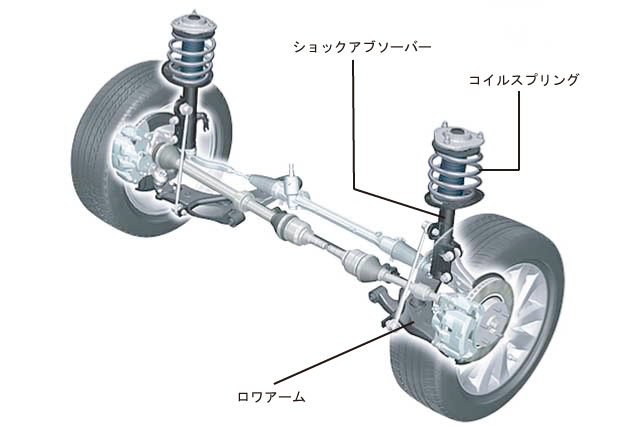
\includegraphics[width=120mm]{img/strat.jpg}
  \caption{ストラット式サスペンション}
  \label{fig:strat}%ここに文章中で使用する名前を指定する
 \end{center}
\end{figure}

\begin{figure}[htbt]
 \begin{center}
  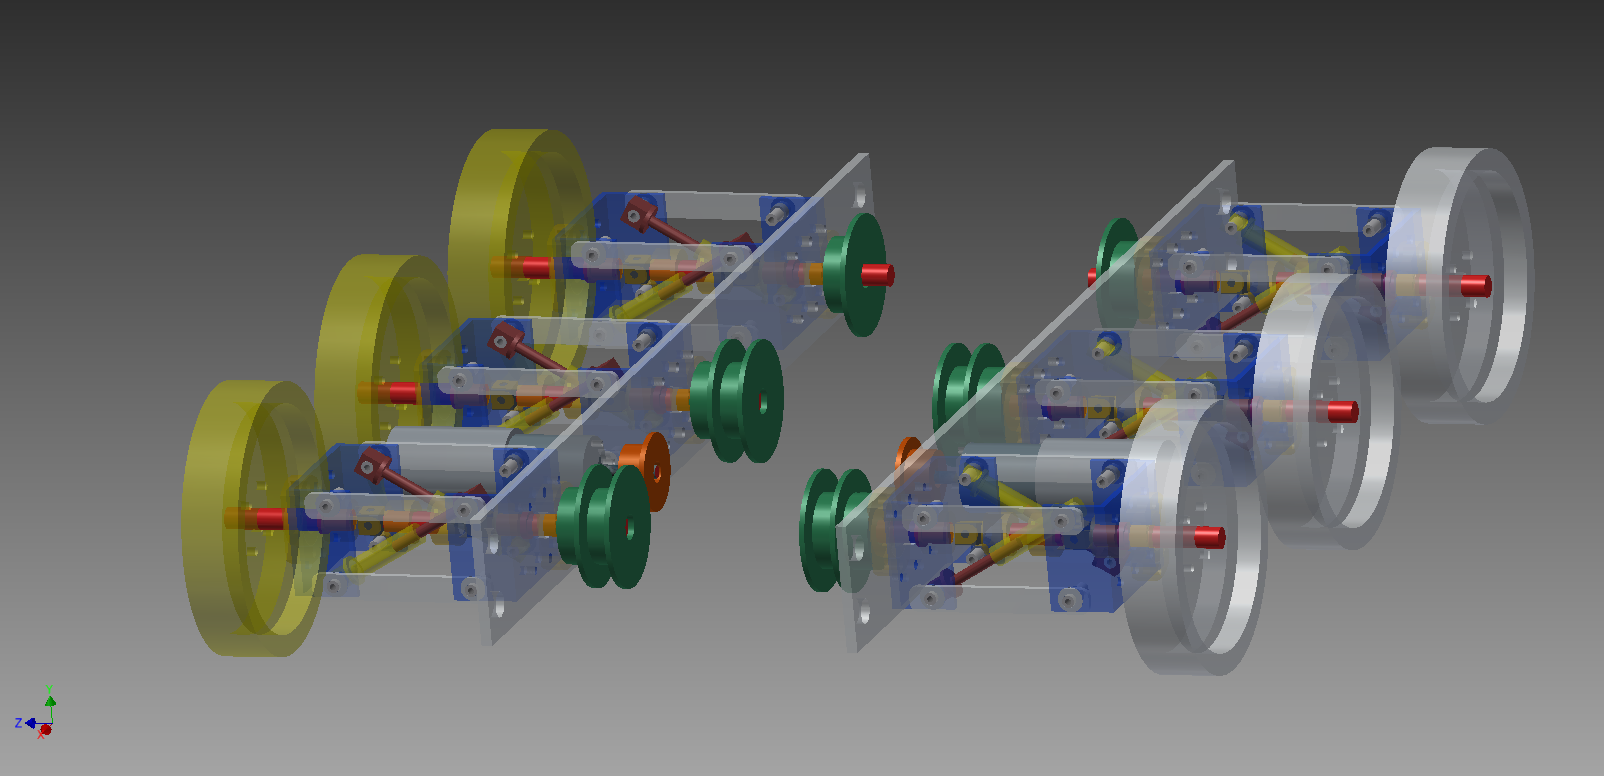
\includegraphics[width=100mm]{img/int.png}
  \caption{6輪ローバ.ここにCAD図でD,Cモジュールで分けた絵を上げる}
  \label{fig:rokurin}%ここに文章中で使用する名前を指定する
 \end{center}
\end{figure}

\begin{figure}[htbt]
 \begin{center}
  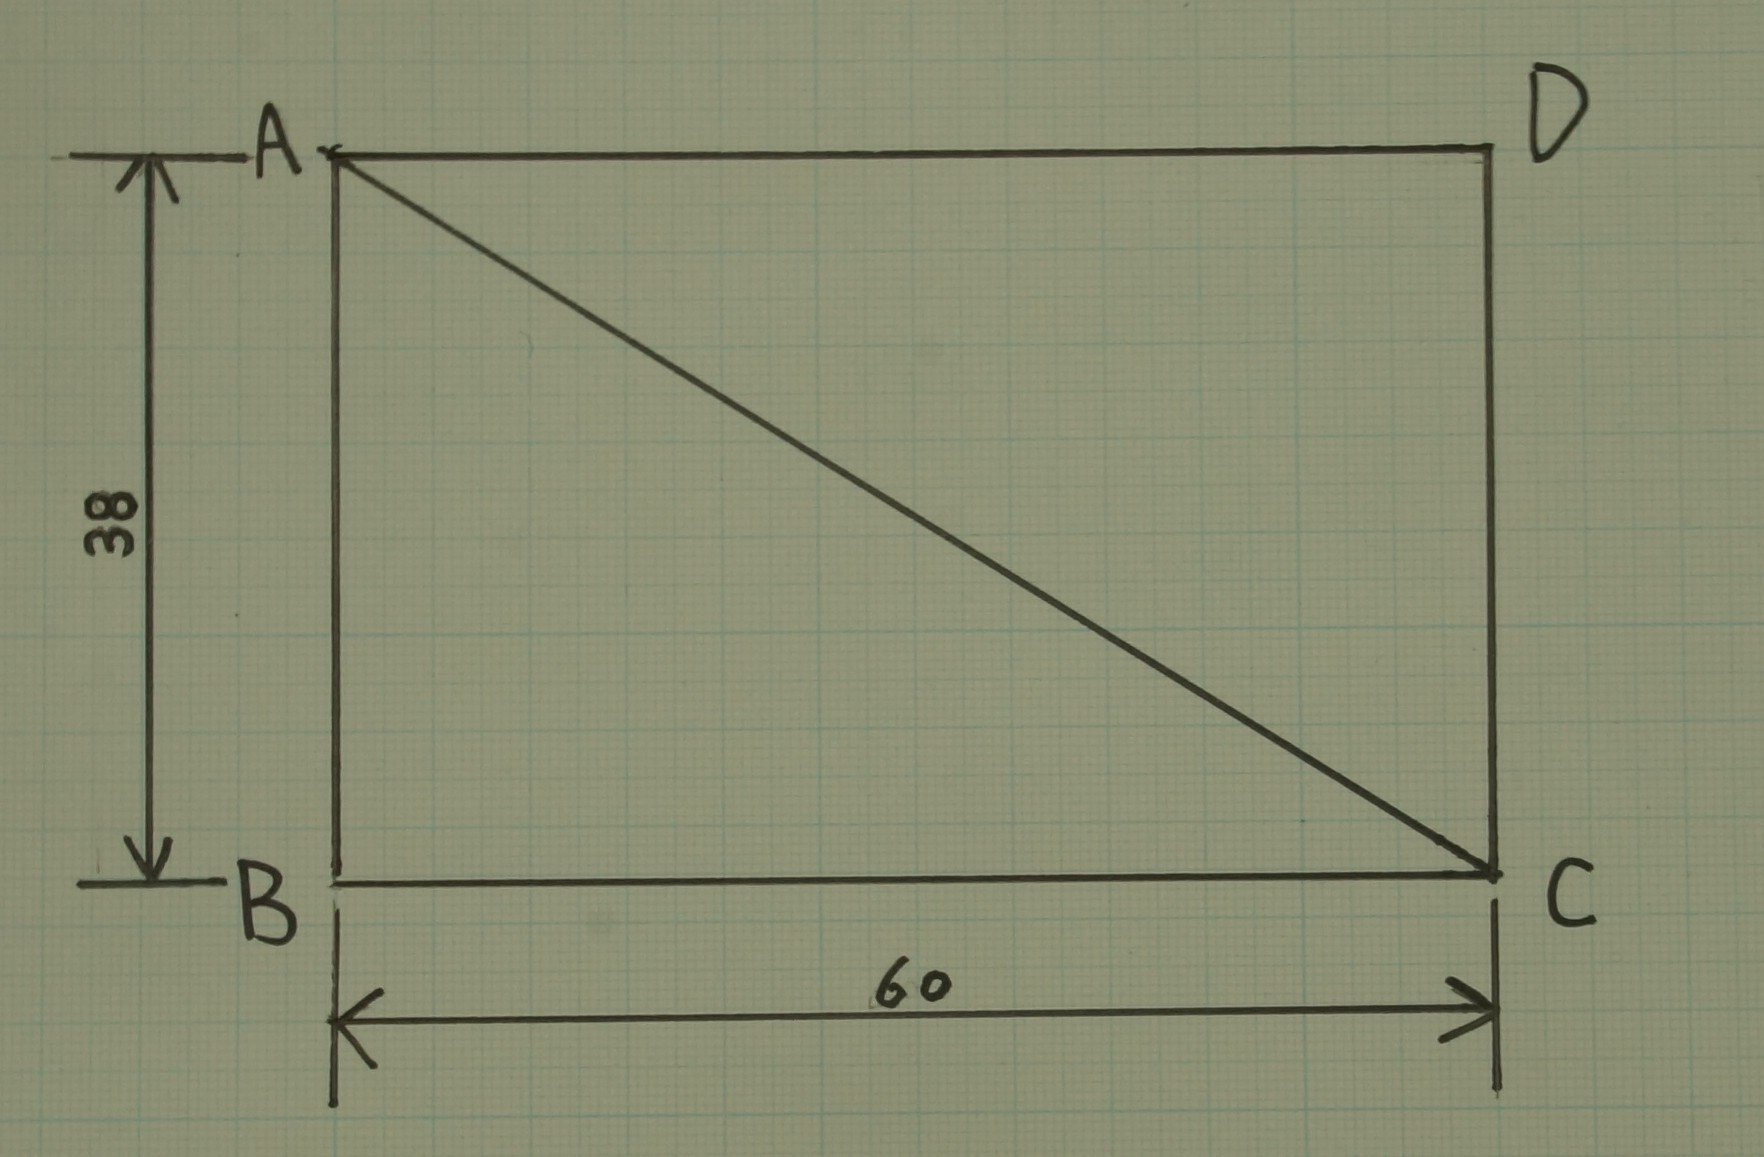
\includegraphics[width=60mm]{img/kanizu.jpg}
  \caption{平行リンク}
  \label{fig:box}%ここに文章中で使用する名前を指定する
 \end{center}
\end{figure}



\begin{figure}[htbt]
 \begin{center}
  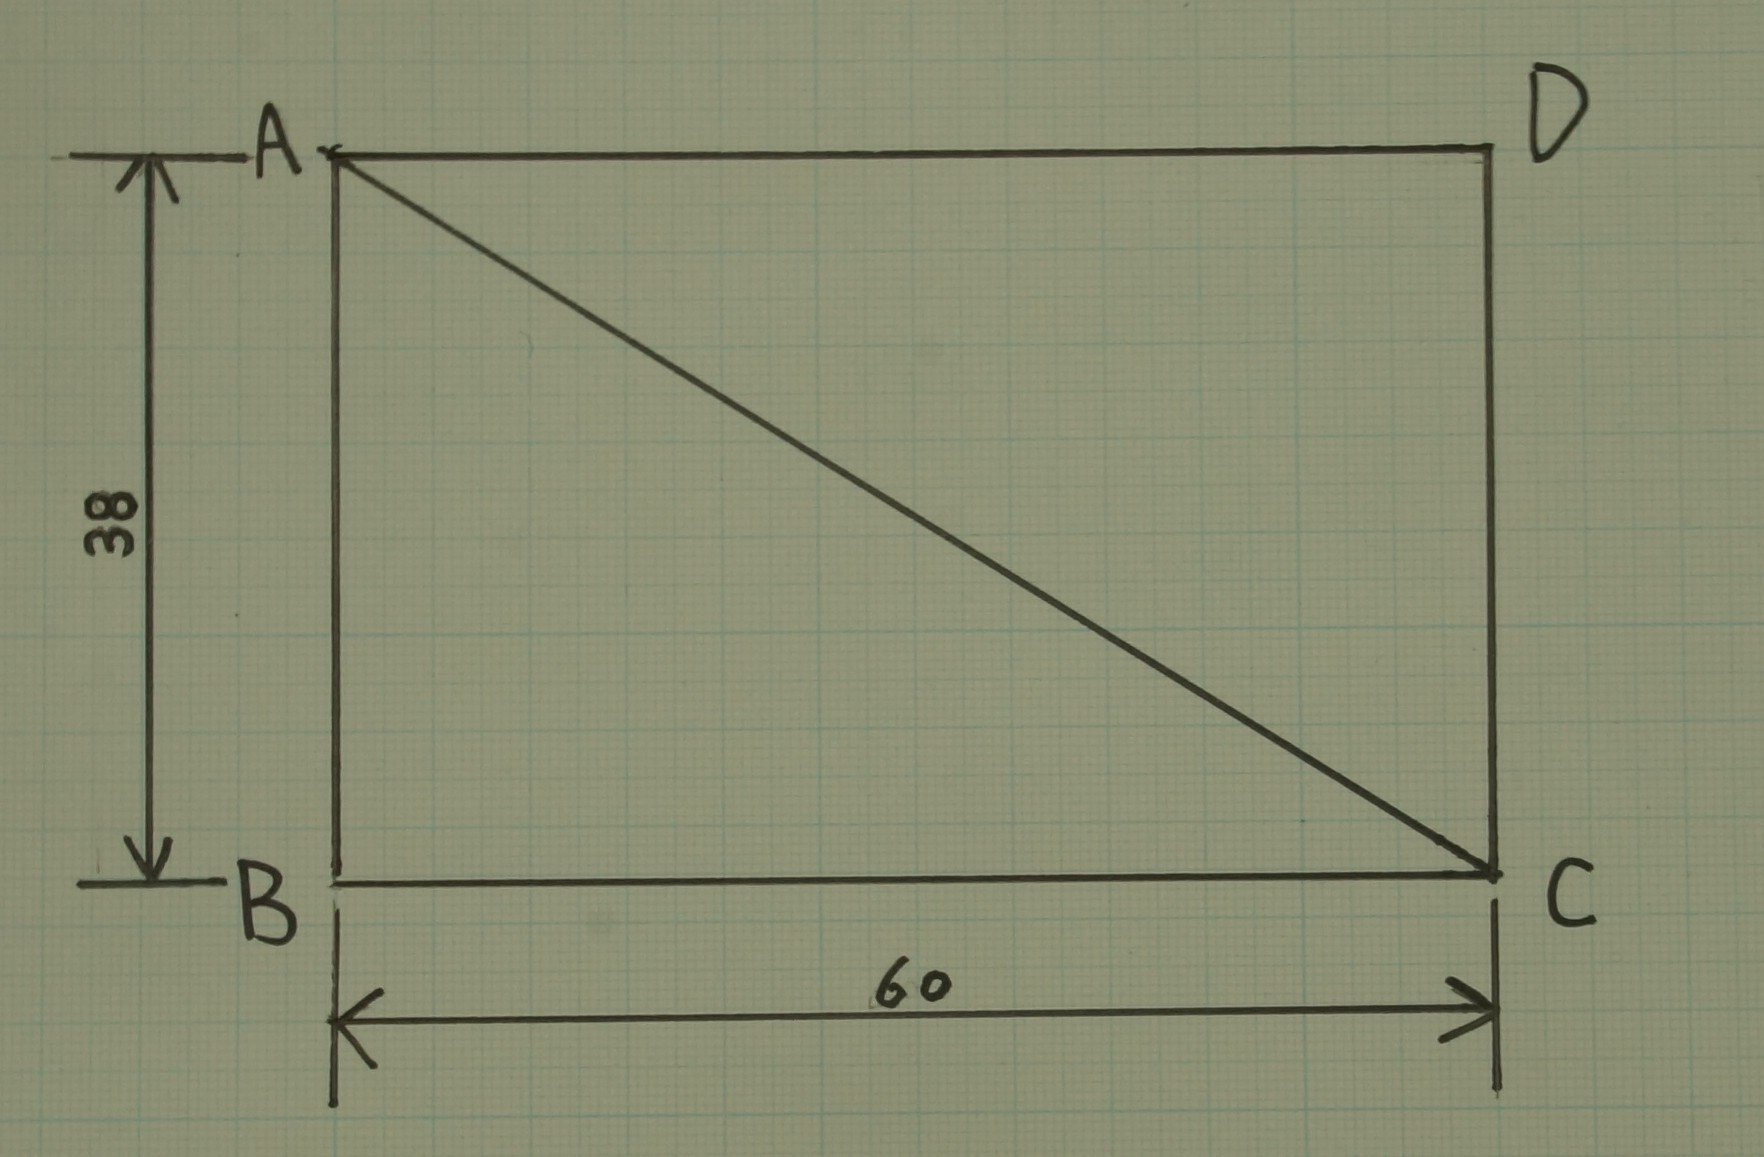
\includegraphics[width=60mm]{img/kanizu.jpg}
  \caption{平行リンク簡易図}
  \label{fig:bix}%ここに文章中で使用する名前を指定する
 \end{center}
\end{figure}


\begin{figure}[htbt]
 \begin{center}
  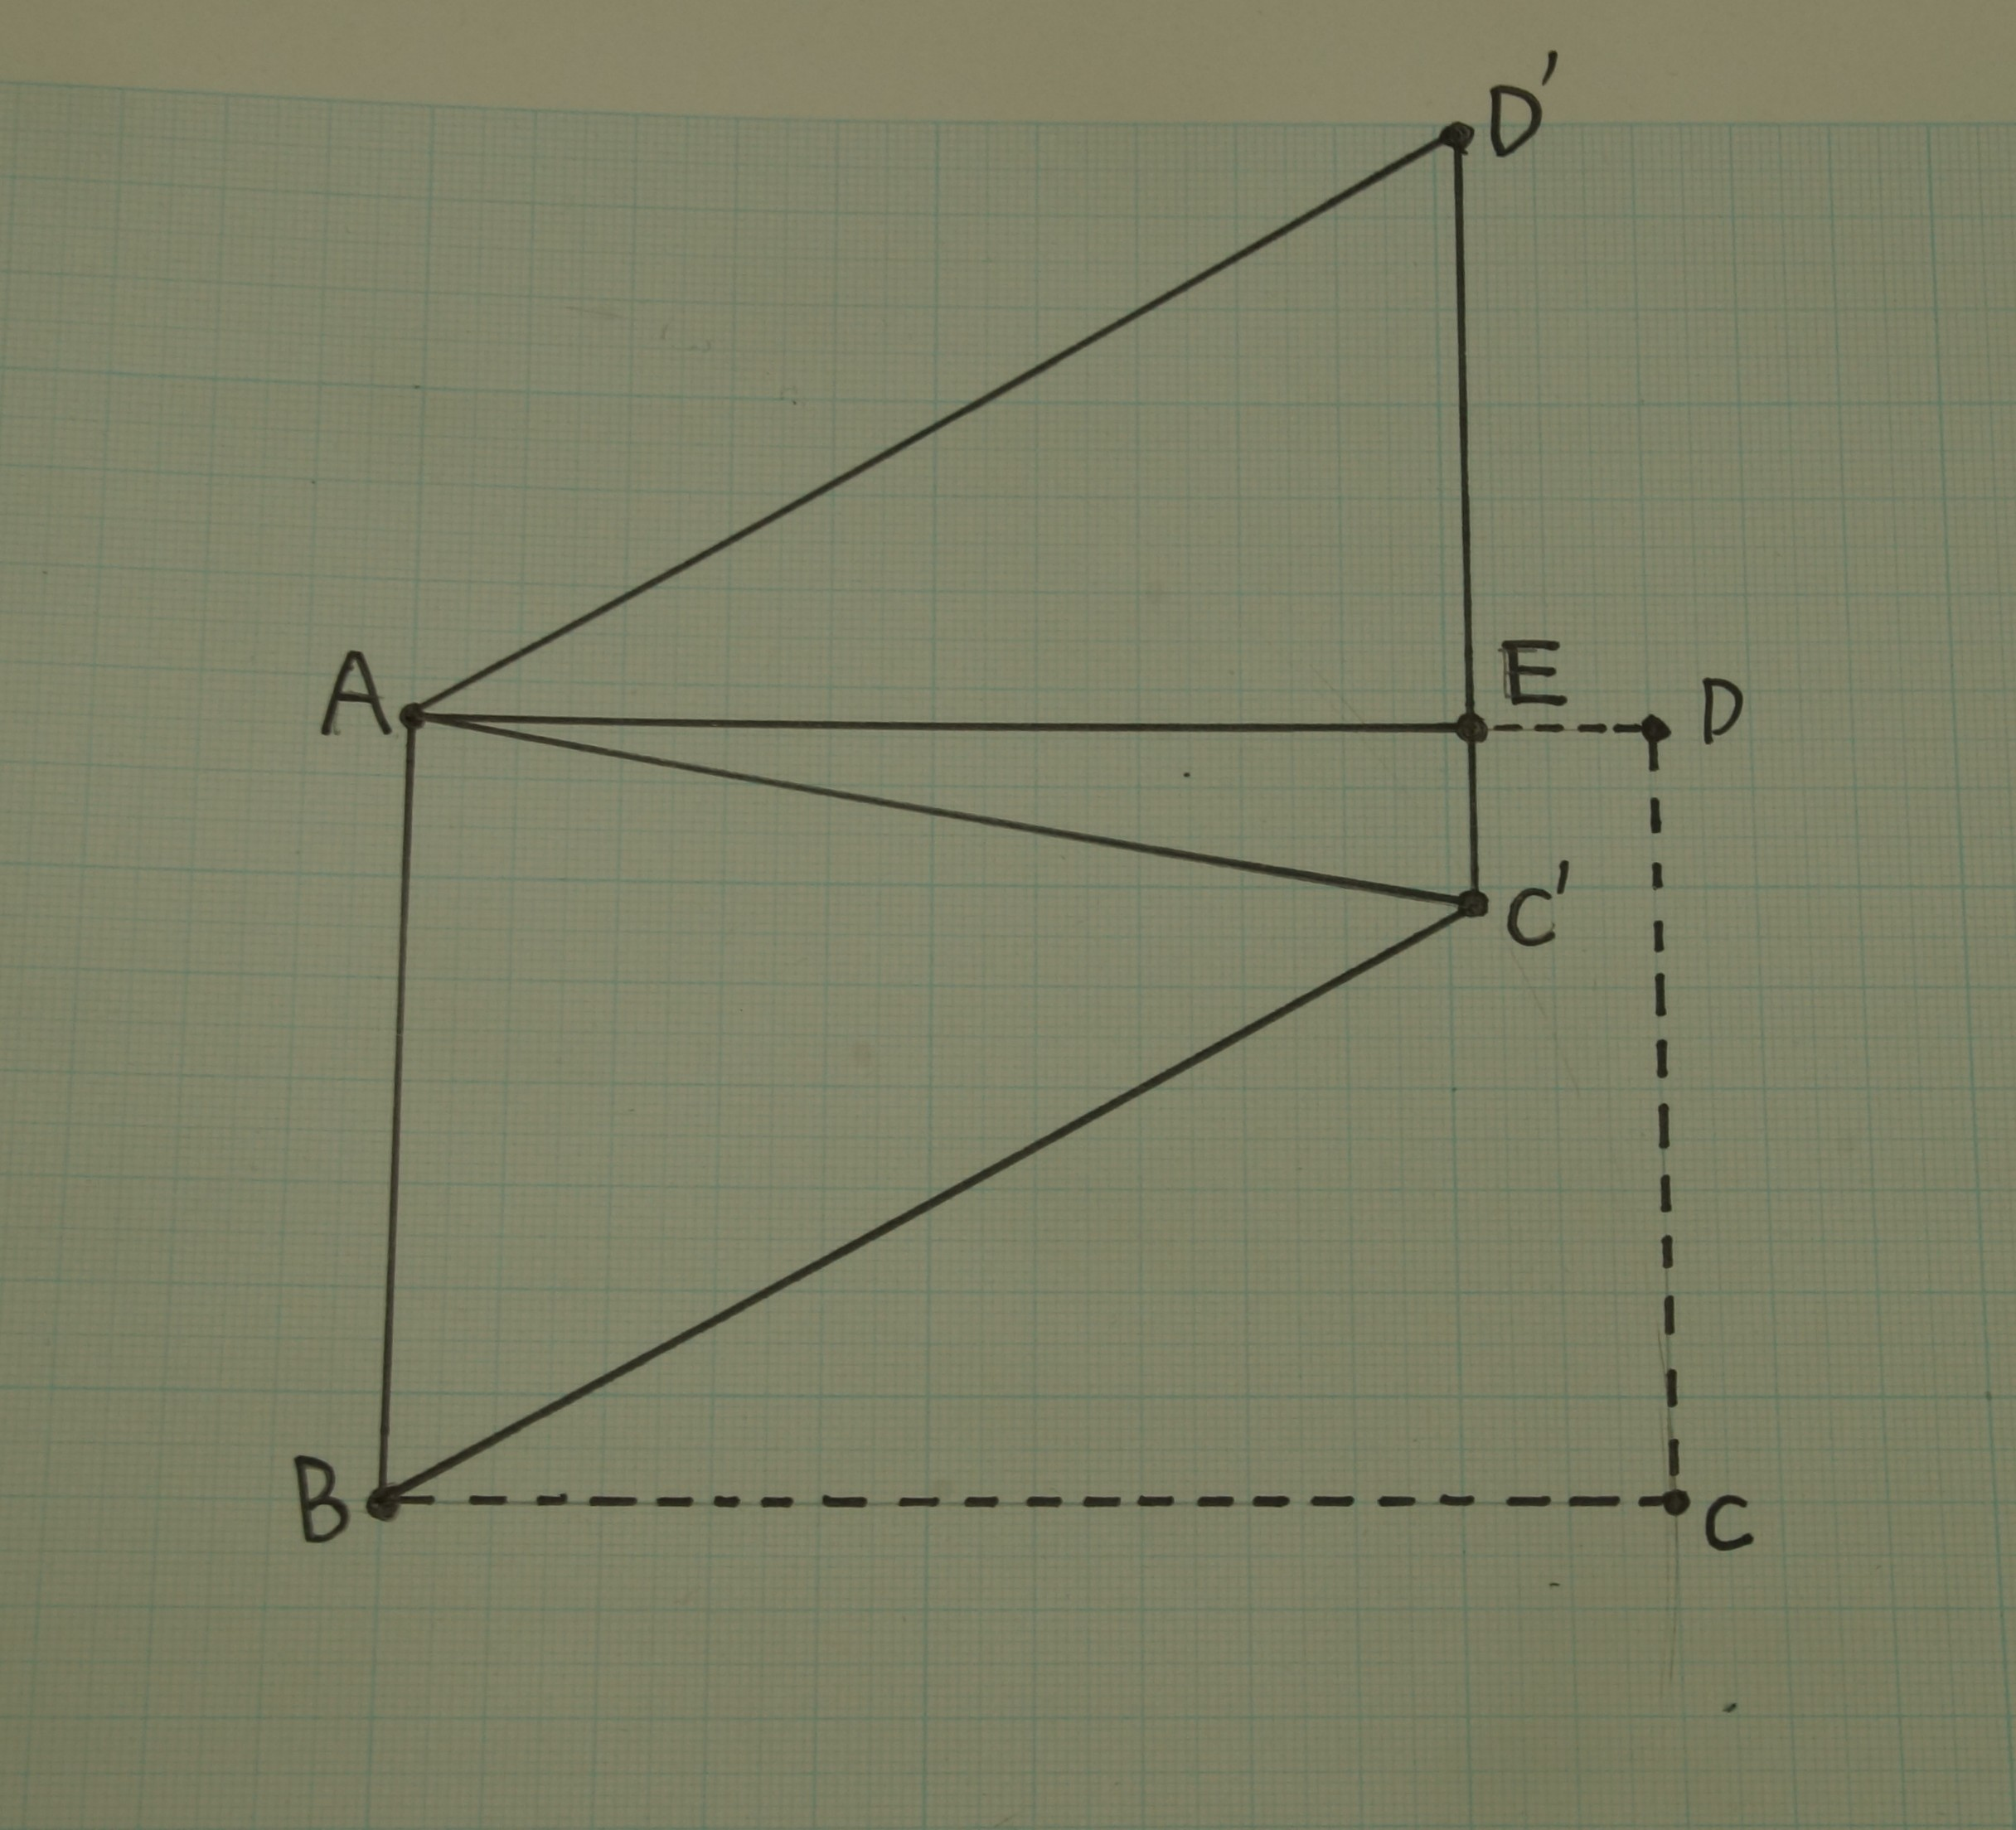
\includegraphics[width=60mm]{img/rink.jpg}
  \caption{平行リンクの移動量変化}
  \label{fig:rink}%ここに文章中で使用する名前を指定する
 \end{center}
\end{figure}


\begin{figure}[htbt]
 \begin{center}
  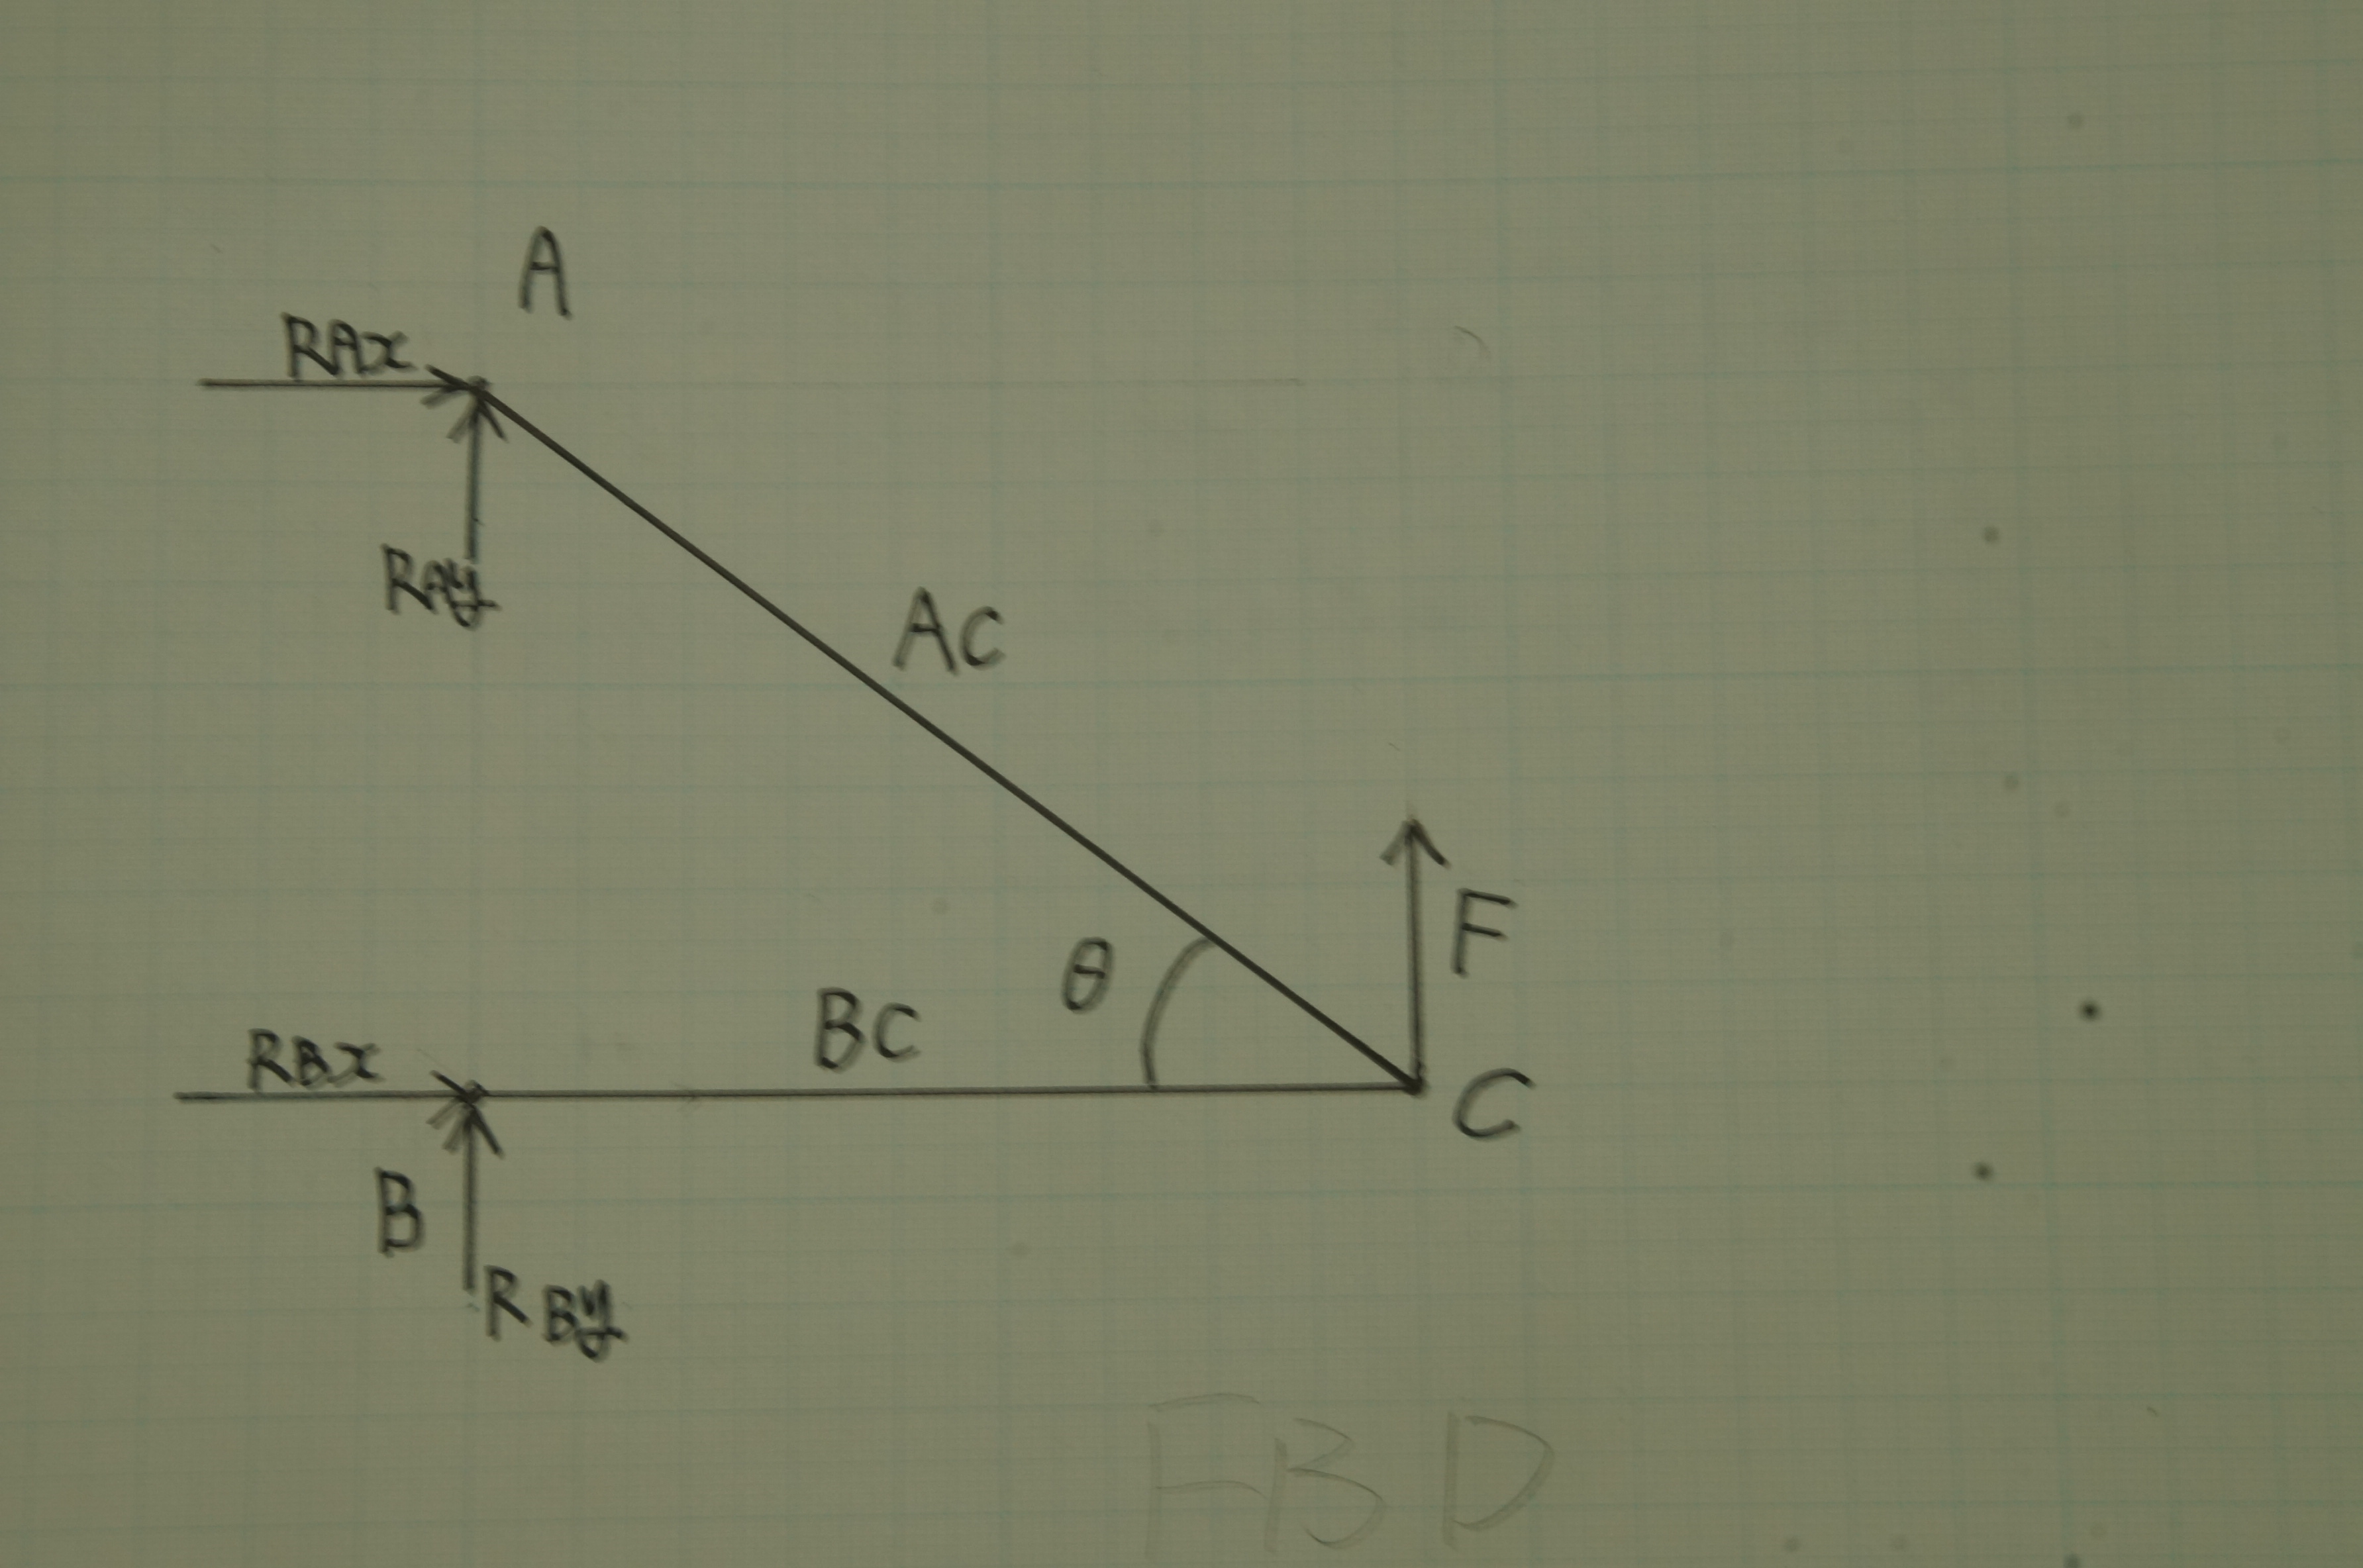
\includegraphics[width=100mm]{img/fbd.jpg}
  \caption{FBD}
  \label{fig:fbd}%ここに文章中で使用する名前を指定する
 \end{center}
\end{figure}


\begin{figure}[htbt]
 \begin{center}
  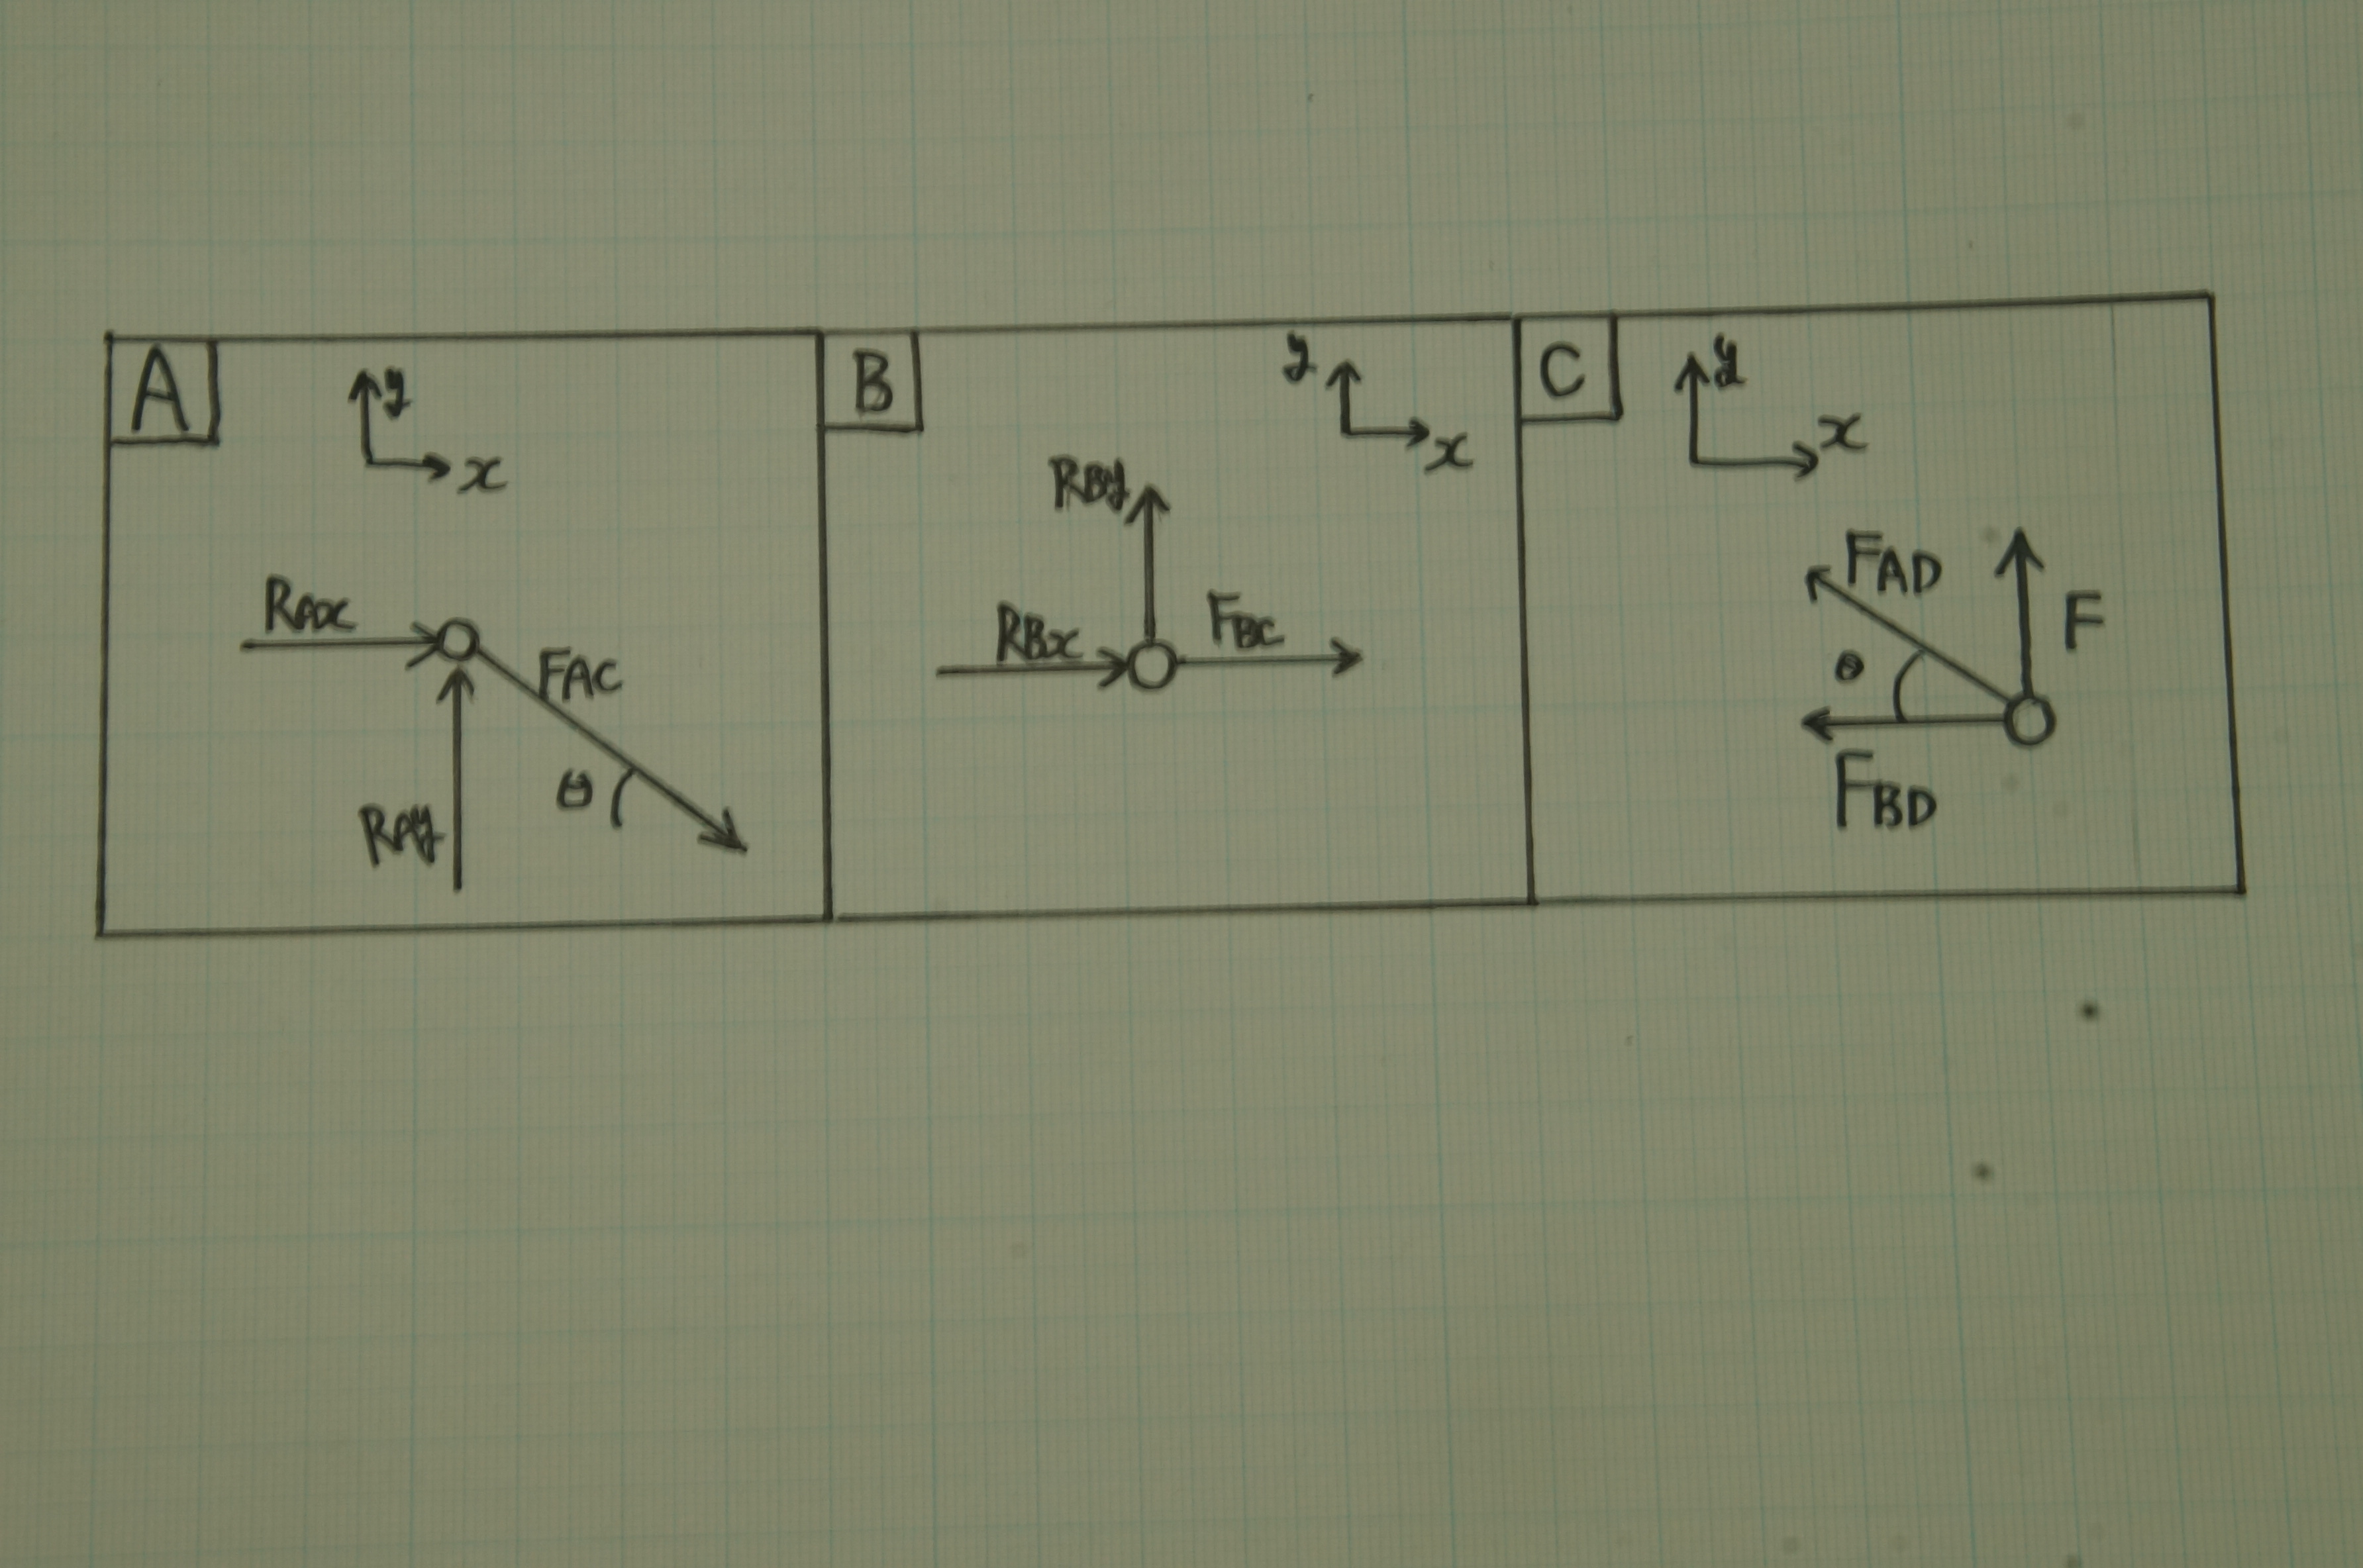
\includegraphics[width=100mm]{img/bai.jpg}
  \caption{各点にかかる力}
  \label{fig:bai}%ここに文章中で使用する名前を指定する
 \end{center}
\end{figure}

\begin{figure}[htbt]
 \begin{center}
  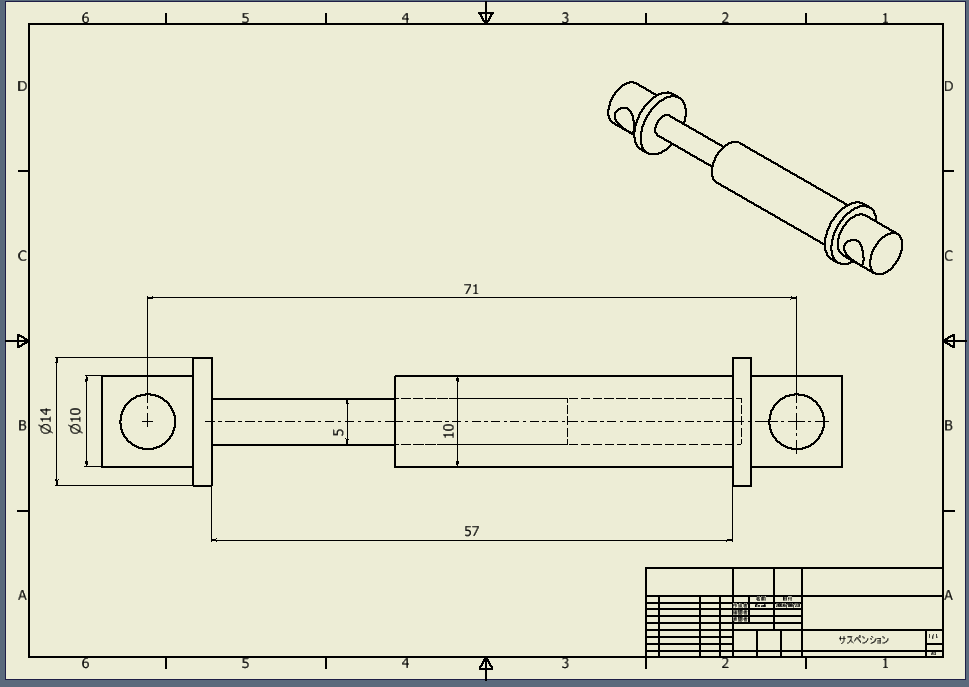
\includegraphics[width=120mm]{img/saspention.png}
  \caption{サスペンションの設計図}
  \label{fig:saspention}%ここに文章中で使用する名前を指定する
 \end{center}
\end{figure}














\end{document}

